
\medskip

\begin{center}
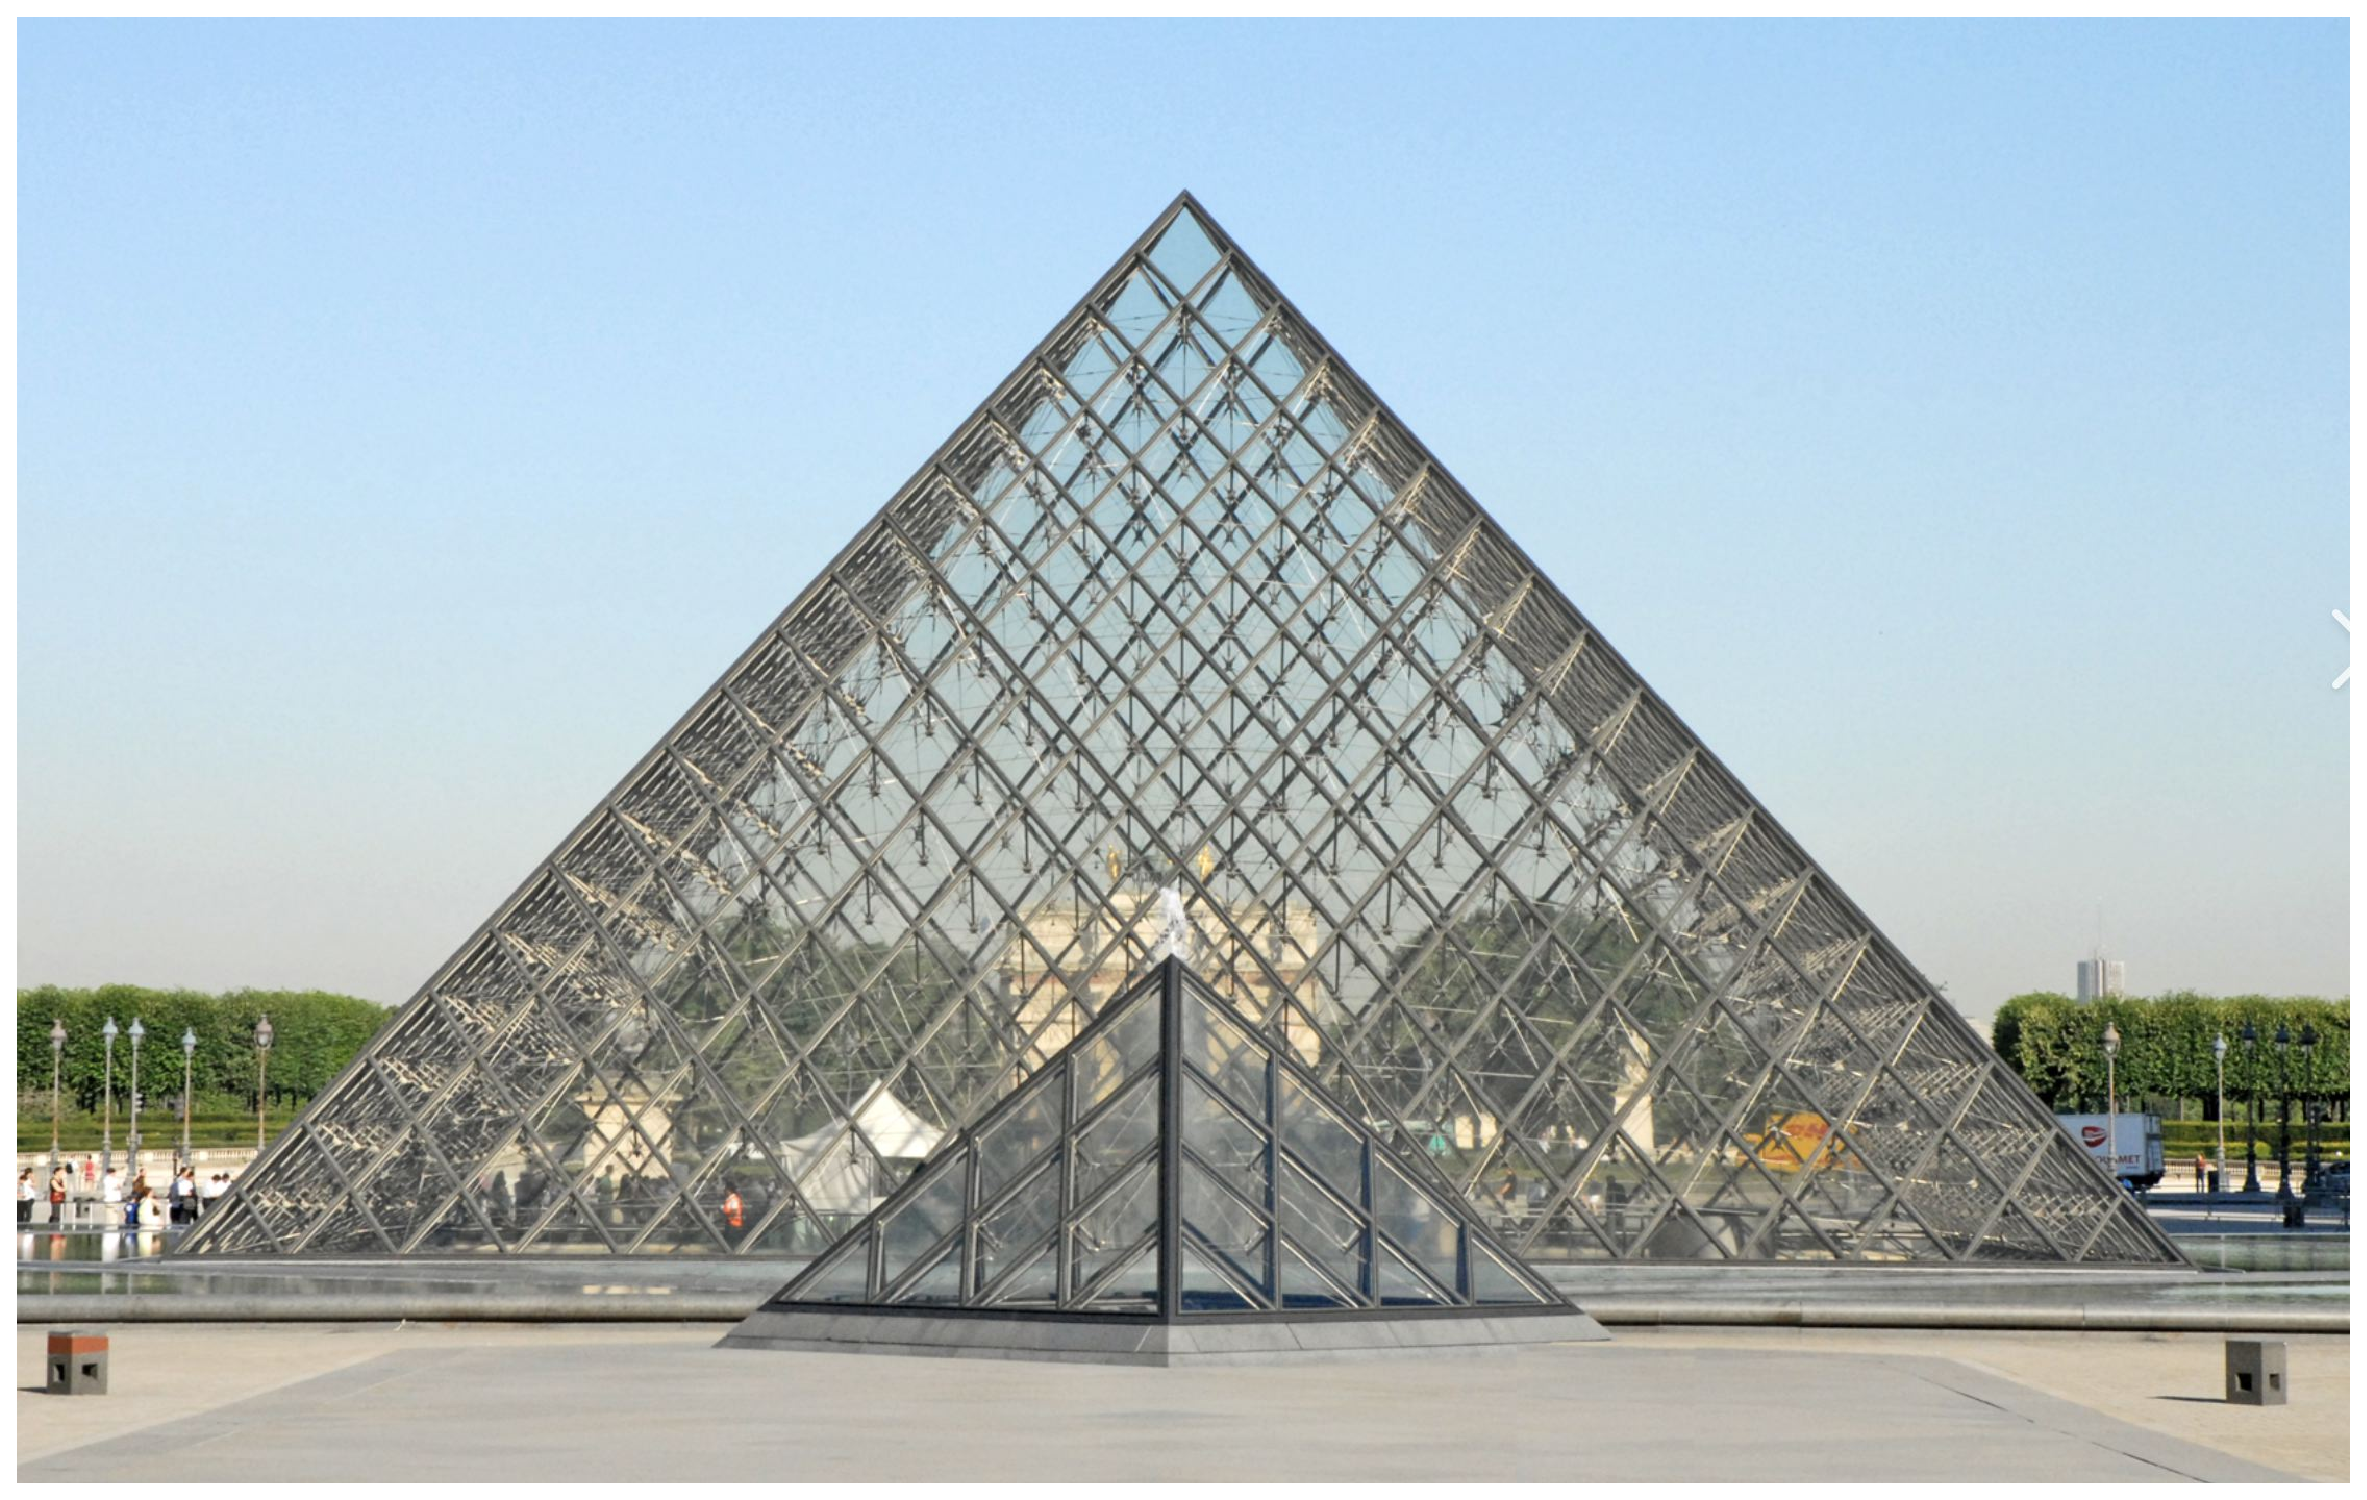
\includegraphics[width=6cm]{pyramide_Polynesie_2019}
\end{center}

La pyramide du Louvre à Paris est une pyramide à base carrée de côté 35,4~m et de hauteur
21,6~m.

C'est une réduction de la pyramide de Khéops en Egypte, qui mesure environ 230,5~m de côté.

\medskip

\begin{enumerate}
\item Montrer que la hauteur de la pyramide de Khéops est d'environ 140,6~m.
\item Calculer le volume en m$^3$ de la pyramide du Louvre. (Arrondir à l'unité)
\item Par quel nombre peut-on multiplier le volume de la pyramide du Louvre pour obtenir celui de la pyramide de Khéops ? (Arrondir à l'unité)
\end{enumerate}

\medskip

\textbf{Rappel:}

Volume d'une pyramide $ =  \dfrac{\text{Aire de la base} \times \text{Hauteur}}{3}$.

\bigskip

